%% ----------------------------------------------------------------------------
%%  §11.9  Appendice: serie di Taylor
%% ----------------------------------------------------------------------------
\section{Appendice: serie di Taylor}
\label{sec:serie-taylor}

Sia $f$ una funzione derivabile infinite volte in un intorno di un punto $x_{0}$. La
formula di Taylor del \cref{cap:taylor} approssima $f$ con polinomi di grado $n$
arbitrario; è naturale chiedersi che cosa accada facendo tendere $n$ all'infinito.

\needspace{14\baselineskip}
\begin{definizione}[Serie di Taylor]\label{def:serie-taylor}\index{serie!di Taylor}
La serie
\begin{equation}\label{eq:serie-taylor}
  \sum_{k=0}^{\infty}\frac{f^{(k)}(x_{0})}{k!}(x-x_{0})^{k}
  =f(x_{0})+f'(x_{0})(x-x_{0})+\frac{f''(x_{0})}2(x-x_{0})^{2}+\cdots
\end{equation}
si chiama \emph{serie di Taylor} di $f$ con centro $x_{0}$ (\emph{serie di Mac Laurin} se
$x_{0}=0$). La funzione $f$ si dice \emph{sviluppabile in serie di Taylor} con centro $x_{0}$
se esiste $\delta>0$ tale che
\begin{equation}\label{eq:sviluppabile}
  f(x)=\sum_{k=0}^{\infty}\frac{f^{(k)}(x_{0})}{k!}(x-x_{0})^{k} \qquad\perogni x:\ \abs{x-x_{0}}<\delta .
\end{equation}
\end{definizione}

La somma parziale $n$-esima della serie di Taylor è il polinomio di Taylor $T_{n}(x)$, e
$f(x)=T_{n}(x)+R_{n}(x)$. Dunque, per un $x$ fissato, \emph{la serie di Taylor converge a
$f(x)$ se e solo se il resto $R_{n}(x)$ tende a zero per $n\to+\infty$}. Si noti che non basta
che la serie converga: deve convergere proprio a $f(x)$. Il resto di Peano, che descrive
$R_{n}$ per $x\to x_{0}$ con $n$ fissato, non dice nulla su questa domanda; servono le stime del
resto del \S\ref{sec:resto-integrale} e del \S\ref{sec:resto-lagrange}.

\begin{teorema}[Sviluppabilità con derivate equilimitate]\label{teo:sviluppabilita}
Sia $f$ derivabile infinite volte nell'intervallo $[x_{0}-\delta,x_{0}+\delta]$, con $\delta>0$, e
supponiamo che esista un numero $M$ tale che
\begin{equation}\label{eq:derivate-equilimitate}
  \abs{f^{(n)}(x)}\le M \qquad\perogni x\in[x_{0}-\delta,x_{0}+\delta],\ \perogni n\in\N .
\end{equation}
Allora $f$ è sviluppabile in serie di Taylor con centro $x_{0}$, e la \eqref{eq:sviluppabile}
vale per ogni $x\in[x_{0}-\delta,x_{0}+\delta]$.
\end{teorema}

\begin{schema}
\Ipotesi{$f\in C^{\infty}([x_{0}-\delta,x_{0}+\delta])$; \ $\abs{f^{(n)}}\le M$ per ogni $n$, con $M$
indipendente da $n$.}
\Tesi{$f(x)=\sum_{k=0}^{\infty}\frac{f^{(k)}(x_{0})}{k!}(x-x_{0})^{k}$ per ogni $x\in[x_{0}-\delta,x_{0}+\delta]$.}
\end{schema}

\begin{strategia}
Basta mostrare che $R_{n}(x)\to0$. La stima del resto (\cref{cor:stima-resto}) dà
$\abs{R_{n}(x)}\le M\frac{\delta^{n+1}}{(n+1)!}$, e il fattoriale al denominatore vince sulla potenza al
numeratore. È essenziale che $M$ non dipenda da $n$.
\end{strategia}

\begin{dimostrazione}
Fissato $x\in[x_{0}-\delta,x_{0}+\delta]$, per il \cref{cor:stima-resto} e l'ipotesi
\eqref{eq:derivate-equilimitate}, con $\abs{x-x_{0}}\le\delta$,
\[
  \abs{R_{n}(x)}\le M\,\frac{\abs{x-x_{0}}^{n+1}}{(n+1)!}\le M\,\frac{\delta^{n+1}}{(n+1)!} .
\]
Per la gerarchia degli infiniti (\cref{teo:gerarchia}) $\frac{\delta^{n+1}}{(n+1)!}\to0$ (se $\delta\le1$
basta maggiorare con $\frac1{(n+1)!}$), e quindi $R_{n}(x)\to0$, cioè $T_{n}(x)=f(x)-R_{n}(x)\to f(x)$.
\end{dimostrazione}

Si noti che la maggiorazione $M\frac{\delta^{n+1}}{(n+1)!}$ \emph{non dipende da $x$}: l'errore commesso
sostituendo $f$ con $T_{n}$ è piccolo, per $n$ grande, contemporaneamente in tutti i punti
dell'intervallo. È il fatto, osservato nel \cref{sec:taylor} per il seno
(\cref{fig:taylor-seno}), che i polinomi di Taylor di grado alto approssimano bene la
funzione su intervalli sempre più ampi.

\begin{notastorica}[Cauchy, Abel e la convergenza uniforme]
Nel \emph{Cours d'analyse} (1821) Cauchy enunciò un teorema in apparenza naturale: se una
serie di funzioni continue converge in ogni punto di un intervallo, la sua somma è
continua. Cinque anni dopo Niels Henrik Abel, nella memoria del 1826 sulla serie
binomiale di Newton, di cui studiava la convergenza anche per esponenti e variabile
complessi, osservò in nota che il teorema «ammette eccezioni»: la serie
$\sen x-\frac12\sen2x+\frac13\sen3x-\cdots$, i cui termini sono funzioni continue, converge per ogni
$x$ e ha somma $\frac x2$ per $-\pi<x<\pi$, ma per $x=\pi$ vale $0$: la somma ha un salto. Serie di
seni e coseni di questo tipo erano al centro della \emph{Théorie analytique de la chaleur}
di Joseph Fourier (1822, con risultati presentati già nel 1807), che vi sviluppava
funzioni qualsiasi, anche discontinue; la serie di Glauert \eqref{eq:glauert} appartiene
alla stessa famiglia. Al teorema di Cauchy manca l'ipotesi che l'errore commesso
troncando la serie sia piccolo \emph{contemporaneamente} in tutti i punti, come accade
nella stima del \cref{teo:sviluppabilita}: è la \emph{convergenza uniforme}. Intravista
negli anni Quaranta da Philipp Seidel e George Stokes, e usata da Cauchy stesso nel 1853
per correggere il proprio enunciato, essa divenne con Karl Weierstrass, che la usava già
nel 1841, uno strumento fondamentale dell'analisi.
\end{notastorica}

\begin{esempio}[Seno, coseno, esponenziale]\label{es:serie-elementari}
Le derivate di $\sen x$ e di $\cos x$ sono $\pm\sen x$ o $\pm\cos x$, e quindi sono limitate da
$M=1$ su qualunque intervallo. Per il \cref{teo:sviluppabilita}, con $x_{0}=0$ e $\delta$
arbitrario, e per gli sviluppi \eqref{eq:taylor-sen}, \eqref{eq:taylor-cos},
\begin{align}
  \sen x&=x-\frac{x^{3}}{3!}+\frac{x^{5}}{5!}-\dots=\sum_{k=0}^{\infty}(-1)^{k}\frac{x^{2k+1}}{(2k+1)!} , \label{eq:serie-seno}\\
  \cos x&=1-\frac{x^{2}}{2}+\frac{x^{4}}{4!}-\dots=\sum_{k=0}^{\infty}(-1)^{k}\frac{x^{2k}}{(2k)!} , \label{eq:serie-coseno}
\end{align}
per ogni $x\in\R$. Per l'esponenziale, $\abs{D^{n}e^{x}}=e^{x}\le e^{\delta}=M$ in $[-\delta,\delta]$; poiché $\delta$
è arbitrario,
\begin{equation}\label{eq:serie-esponenziale}
  e^{x}=1+x+\frac{x^{2}}{2!}+\dots+\frac{x^{n}}{n!}+\dots=\sum_{k=0}^{\infty}\frac{x^{k}}{k!} \qquad\perogni x\in\R ,
\end{equation}
che per $x=1$ ritrova la \eqref{eq:e-serie}. Le tre serie convergono assolutamente per ogni
$x$: l'esponenziale per l'\cref{es:assoluta}, il seno e il coseno per confronto con la
serie $\sum\frac{\abs x^{k}}{k!}$.
\end{esempio}

\needspace{12\baselineskip}
\begin{osservazione}[L'esponenziale definito da una serie]\label{oss:exp-serie}
Nel \cref{cap:numeri} avevamo annunciato una definizione alternativa delle potenze a
esponente reale. Eccola: si può \emph{definire} la funzione esponenziale mediante la
serie, $\exp x=\sum_{k=0}^{\infty}\frac{x^{k}}{k!}$, che converge per ogni $x$ reale, e poi porre
$a^{b}=\exp(b\log a)$ per $a>0$. Per la \eqref{eq:serie-esponenziale} e la relazione
$a^{b}=e^{b\log a}$ \eqref{eq:potenza-esponenziale}, questa definizione coincide con quella
data mediante l'estremo superiore. Molti testi seguono la strada inversa e costruiscono
tutta la teoria di esponenziali e logaritmi a partire dalla serie: la proprietà
fondamentale $\exp(x+y)=\exp x\cdot\exp y$ richiede allora di saper moltiplicare due serie
(il \emph{prodotto di Cauchy}), argomento dei corsi successivi.
\end{osservazione}

\subsection{Logaritmo e arcotangente}

Anche la serie geometrica è una serie di Taylor: per $f(x)=\frac1{1-x}$ si ha
$f^{(n)}(x)=\frac{n!}{(1-x)^{n+1}}$, cioè $\frac{f^{(n)}(0)}{n!}=1$, e il \cref{teo:serie-geometrica} dice che
$\frac1{1-x}=\sum_{k=0}^{\infty}x^{k}$ per $\abs x<1$. Il resto è esplicito,
$\frac1{1-x}-\sum_{k=0}^{n}x^{k}=\frac{x^{n+1}}{1-x}$, e integrandolo (con $-t$ o $-t^{2}$ al posto di $x$) abbiamo
ottenuto nel \S\ref{sec:taylor-peano} gli sviluppi del logaritmo e dell'arcotangente con
il resto in forma esplicita. Per queste funzioni le derivate non sono equilimitate, ma
il resto si può studiare direttamente.

\begin{proposizione}[Serie del logaritmo e dell'arcotangente]\label{prop:serie-log-arctg}
\begin{align}
  \log(1+x)&=\sum_{k=1}^{\infty}(-1)^{k-1}\frac{x^{k}}k=x-\frac{x^{2}}2+\frac{x^{3}}3-\cdots
  && (-1<x\le1), \label{eq:serie-log}\\
  \operatorname{arctg}x&=\sum_{k=0}^{\infty}(-1)^{k}\frac{x^{2k+1}}{2k+1}=x-\frac{x^{3}}3+\frac{x^{5}}5-\cdots
  && (-1\le x\le1). \label{eq:serie-arctg}
\end{align}
Per $\abs x>1$ entrambe le serie non convergono.
\end{proposizione}

\begin{schema}
\Ipotesi{$-1<x\le1$ per il logaritmo, $-1\le x\le1$ per l'arcotangente; \ $\abs x>1$ per
l'ultima affermazione.}
\Tesi{le somme parziali delle due serie tendono a $\log(1+x)$ e a $\operatorname{arctg}x$;
\ per $\abs x>1$ le serie non convergono.}
\end{schema}

\begin{strategia}
Per entrambe le funzioni il resto è stato ottenuto integrando il resto esplicito della
progressione geometrica, e ne conosciamo una maggiorazione: basta verificare che tende a
zero per $n\to+\infty$ quando $\abs x\le1$ (escluso $x=-1$ per il logaritmo, dove la funzione non
è definita). Per $\abs x>1$ si usa la condizione necessaria.
\end{strategia}

\begin{dimostrazione}
Per il logaritmo, nel \S\ref{sec:taylor-peano} abbiamo trovato
$\abs{R_{n}(x)}\le\frac{x^{n+1}}{n+1}$ per $0\le x\le1$ e $\abs{R_{n}(x)}\le\frac{\abs x^{n+1}}{(n+1)(1+x)}$ per $-1<x<0$; in
entrambi i casi $R_{n}(x)\to0$, perché $\abs x\le1$ e $\frac1{n+1}\to0$. Per l'arcotangente, la
\cref{prop:sviluppo-arctg} dà $\abs{R(x)}\le\frac{\abs x^{2n+3}}{2n+3}\to0$ per $\abs x\le1$. Se infine
$\abs x>1$, i termini $\frac{\abs x^{k}}k$ e $\frac{\abs x^{2k+1}}{2k+1}$ tendono a $+\infty$ (gerarchia degli
infiniti), e le serie non convergono per la condizione necessaria.
\end{dimostrazione}

Con $x=1$ si ritrovano le somme $\log2$ della serie armonica alternata e $\frac\pi4$ della
serie di Leibniz. Le due serie convergono però lentamente; per calcolare davvero $\log2$
conviene un'altra serie. Sottraendo dalla \eqref{eq:serie-log} la stessa formula con $-x$
al posto di $x$ (\cref{prop:linearita-serie}), per $\abs x<1$ i termini di grado pari si
elidono e
\begin{equation}\label{eq:serie-log-rapporto}
  \log\frac{1+x}{1-x}=2\Bigl(x+\frac{x^{3}}3+\frac{x^{5}}5+\cdots\Bigr)=2\sum_{k=0}^{\infty}\frac{x^{2k+1}}{2k+1} .
\end{equation}
Con $x=\frac13$ si ottiene $\frac{1+x}{1-x}=2$: la serie ha i termini dell'ordine di $9^{-k}$, e dieci
termini danno $\log2$ con un errore dell'ordine di $10^{-11}$, mentre dieci termini della
serie armonica alternata danno a stento la prima cifra decimale (errore $\approx5\cdot10^{-2}$). È lo stesso principio della formula di Machin
per $\pi$. Con il resto integrale, la \cref{prop:sviluppo-log-rapporto} del
\cref{cap:taylor} dà anche una stima esplicita dell'errore, ed è il punto di partenza per
costruire un'intera tavola di logaritmi.

\begin{osservazione}[Il raggio di convergenza]\label{oss:raggio-convergenza}
\index{raggio di convergenza}
Le serie di questo paragrafo sono \emph{serie di potenze} $\sum_{k=0}^{\infty}c_{k}x^{k}$ (con centro $0$;
per un centro $x_{0}$ basta scrivere $x-x_{0}$ al posto di $x$), e l'insieme degli $x$ in cui
convergono ha una struttura semplice. Se la serie converge in un punto $y\neq0$, i
termini $c_{k}y^{k}$ tendono a zero e sono quindi limitati, $\abs{c_{k}y^{k}}\le M$; per $\abs x<\abs y$
si ha allora $\abs{c_{k}x^{k}}\le M\abs{x/y}^{k}$, e per il confronto con una serie geometrica la
serie converge assolutamente in $x$ (\emph{lemma di Abel}). Posto
$r=\sup\{\abs y\tc\text{la serie converge in }y\}\in[0,+\infty]$, la serie converge dunque
assolutamente per $\abs x<r$ e, per definizione di $r$, non converge per $\abs x>r$; negli
estremi $x=\pm r$ può accadere di tutto. Il numero $r$ si chiama \emph{raggio di
convergenza}: nel campo complesso l'insieme $\abs z<r$ è un disco, e il nome viene di lì.

Quando esiste $L=\lim\frac{\abs{c_{k+1}}}{\abs{c_{k}}}$ (con $c_{k}\neq0$) oppure $L=\lim\sqrt[k]{\abs{c_{k}}}$, il
raggio si calcola con il \cref{cor:rapporto-assoluto}: per i termini $c_{k}x^{k}$ il limite
corrispondente vale $L\abs x$, e quindi $r=\frac1L$, con $r=+\infty$ se $L=0$ e $r=0$ se $L=+\infty$.
Così la serie esponenziale ha $r=+\infty$, quella del logaritmo $r=1$; per l'arcotangente,
che ha nulli i coefficienti di indice pari, si applica il criterio direttamente ai
termini non nulli, il cui rapporto tende a $x^{2}$, e si trova ancora $r=1$. La serie
$\sum\frac{x^{k}}k$ dell'\cref{es:serie-xk-su-k} ha $r=1$, converge in $-1$ e non in $1$.
Quando nessuno dei due limiti esiste, il raggio si calcola con il massimo limite
(\S\ref{subsec:massimo-minimo-limite}): vale sempre la \emph{formula di
Cauchy--Hadamard}\index{formula di Cauchy--Hadamard}
$\frac1r=\limsup_{k}\sqrt[k]{\abs{c_{k}}}$ (con le convenzioni $\frac10=+\infty$ e
$\frac1{+\infty}=0$, e il massimo limite $+\infty$ per le successioni non limitate
superiormente), che qui non dimostriamo.
\end{osservazione}

\subsection{Una funzione non sviluppabile}

Ci si potrebbe aspettare che ogni funzione derivabile infinite volte sia sviluppabile in
serie di Taylor. Non è così, e il controesempio, dovuto a Cauchy, è istruttivo.

\begin{proposizione}[Controesempio di Cauchy]\label{prop:cauchy-controesempio}
La funzione
\begin{equation}\label{eq:cauchy-controesempio}
  f(x)=\begin{cases} e^{-1/x^{2}} & \text{se } x\neq0,\\ 0 & \text{se } x=0 \end{cases}
\end{equation}
è derivabile infinite volte in $\R$, e $f^{(n)}(0)=0$ per ogni $n$. Dunque la sua serie di
Mac Laurin è identicamente nulla e converge a $f(x)$ soltanto per $x=0$: $f$ non è
sviluppabile in serie di Taylor con centro $0$.
\end{proposizione}

\begin{schema}
\Ipotesi{$f$ definita dalla \eqref{eq:cauchy-controesempio}.}
\Tesi{$f\in C^{\infty}(\R)$; \ $f^{(n)}(0)=0$ per ogni $n$; \ $f(x)\neq0=\sum\frac{f^{(k)}(0)}{k!}x^{k}$ per
$x\neq0$.}
\end{schema}

\begin{strategia}
Per $x\neq0$ le derivate si calcolano con le regole usuali, e per induzione hanno tutte
la forma $P(\frac1x)\,e^{-1/x^{2}}$, con $P$ polinomio. Il punto delicato è l'origine: lì la
funzione è «infinitamente piatta», perché $e^{-1/x^{2}}$ tende a zero più rapidamente di
qualunque potenza di $x$. Dimostreremo per induzione che ogni derivata esiste in $0$ e
vale $0$, calcolando il limite del rapporto incrementale.
\end{strategia}

\begin{dimostrazione}
\emph{Primo passo: un limite.} Per ogni intero $m\ge0$,
\begin{equation}\label{eq:piatta}
  \lim_{x\to0}\frac{e^{-1/x^{2}}}{\abs x^{m}}=0 .
\end{equation}
Infatti, posto $u=\frac1{x^{2}}\to+\infty$, il quoziente vale $u^{m/2}e^{-u}$, che tende a $0$ per la
\eqref{eq:hopital-potenza-exp} (per $m=0$ è ovvio) e il teorema sul limite delle funzioni
composte. Ne segue che $Q(\frac1x)\,e^{-1/x^{2}}\to0$ per $x\to0$, per ogni polinomio $Q$: è una
combinazione lineare di termini del tipo $\frac{e^{-1/x^{2}}}{x^{m}}$.

\emph{Secondo passo: le derivate per $x\neq0$.} Dimostriamo per induzione che per $x\neq0$
si ha $f^{(n)}(x)=P_{n}(\frac1x)\,e^{-1/x^{2}}$, con $P_{n}$ polinomio. Per $n=0$, $P_{0}=1$. Se la
formula vale per $n$, derivando con la regola del prodotto e quella delle funzioni
composte, e ricordando che $D\frac1x=-\frac1{x^{2}}$ e $D\bigl(-\frac1{x^{2}}\bigr)=\frac2{x^{3}}$,
\[
  f^{(n+1)}(x)=\Bigl[-\frac1{x^{2}}P_{n}'\Bigl(\frac1x\Bigr)+\frac2{x^{3}}P_{n}\Bigl(\frac1x\Bigr)\Bigr]e^{-1/x^{2}}
  =P_{n+1}\Bigl(\frac1x\Bigr)e^{-1/x^{2}} ,
\]
con $P_{n+1}(t)=-t^{2}P_{n}'(t)+2t^{3}P_{n}(t)$, che è un polinomio.

\emph{Terzo passo: le derivate in $0$.} Dimostriamo per induzione che $f^{(n)}(0)$ esiste e
vale $0$. Per $n=0$ è la definizione. Se $f^{(n)}(0)=0$, il rapporto incrementale di $f^{(n)}$
in $0$ è
\[
  \frac{f^{(n)}(x)-f^{(n)}(0)}{x}=\frac1x\,P_{n}\Bigl(\frac1x\Bigr)e^{-1/x^{2}} ,
\]
cioè $Q(\frac1x)e^{-1/x^{2}}$ con $Q(t)=tP_{n}(t)$, che tende a $0$ per il primo passo. Dunque
$f^{(n+1)}(0)=0$. In particolare ogni $f^{(n)}$ è derivabile in tutto $\R$, e quindi $f$ è
derivabile infinite volte. Infine la serie di Mac Laurin di $f$ ha tutti i coefficienti
nulli, e la sua somma è $0\neq e^{-1/x^{2}}=f(x)$ per ogni $x\neq0$.
\end{dimostrazione}

\begin{figure}[htb]
\centering
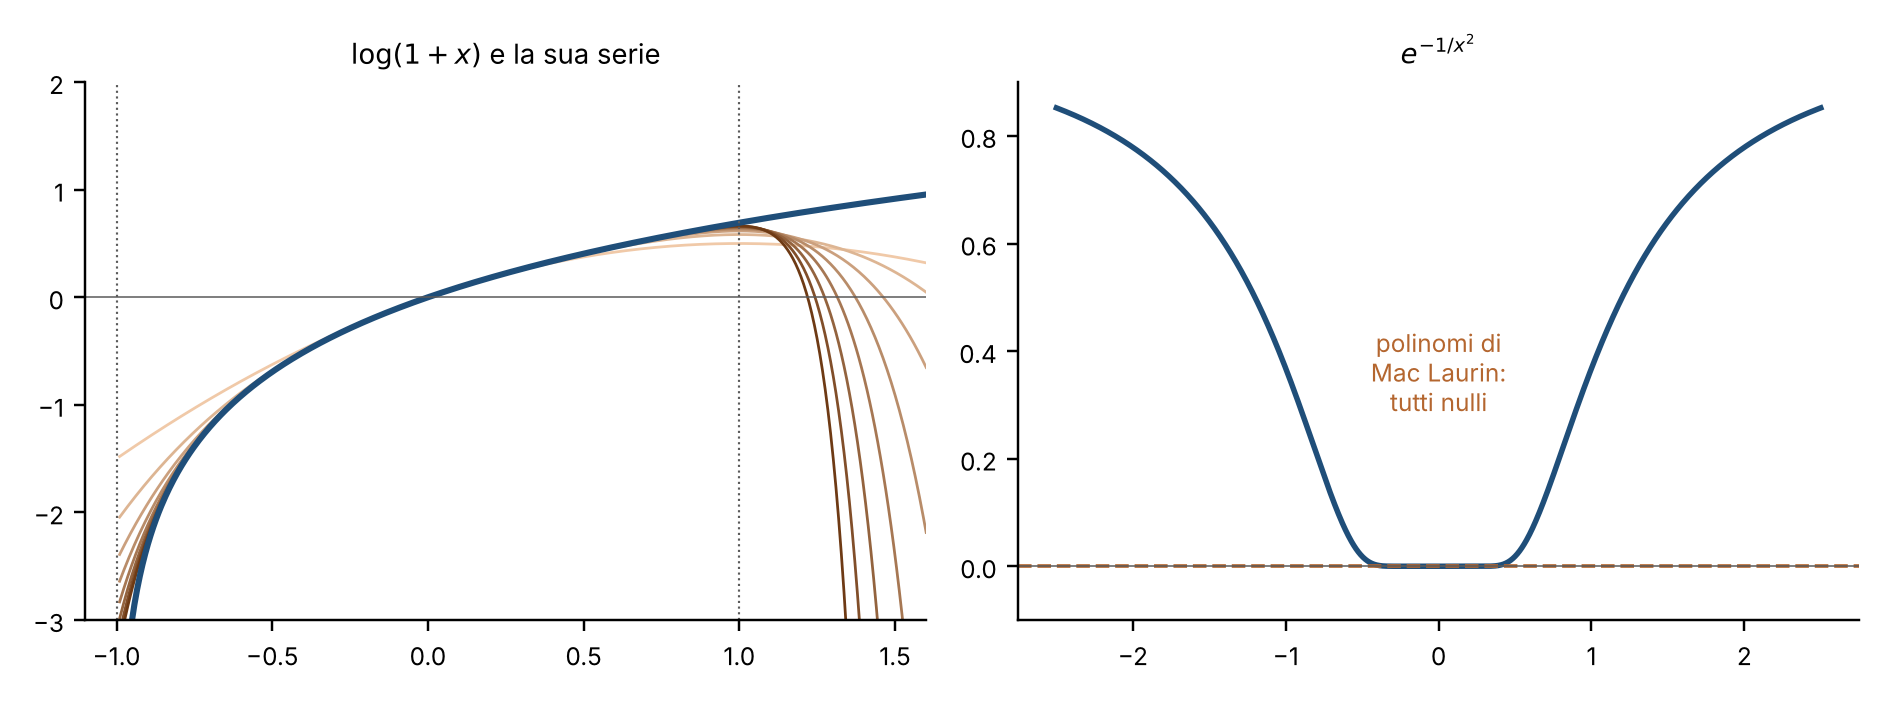
\includegraphics[width=\textwidth]{figure/serie_taylor.png}
\caption{A sinistra: $\log(1+x)$ (blu) e le somme parziali della sua serie di Mac Laurin di
grado $2,4,\dots,16$ (rame): in $(-1,1]$ esse convergono alla funzione, per $x>1$ si
allontanano. A destra: la funzione di Cauchy $e^{-1/x^{2}}$, così piatta nell'origine che tutti
i suoi polinomi di Mac Laurin sono nulli (\texttt{python/fig\_serie\_taylor.py}).}
\label{fig:serie-taylor}
\end{figure}

\subsection{La formula di Eulero}

Nel \cref{cap:complementi} abbiamo introdotto la notazione $e^{i\vartheta}=\cos\vartheta+i\sen\vartheta$
\eqref{eq:eulero}, promettendo di mostrare che si tratta in realtà di un teorema. Le serie
permettono di mantenere la promessa. Diciamo che una successione di numeri complessi
$z_{n}=x_{n}+iy_{n}$ converge a $z=x+iy$ se $x_{n}\to x$ e $y_{n}\to y$, e che una serie di numeri
complessi converge se convergono le sue somme parziali. Poiché la serie esponenziale
\eqref{eq:serie-esponenziale} converge per ogni $x$ reale, è naturale \emph{definire}
l'esponenziale di un numero complesso $z$ come
\begin{equation}\label{eq:esponenziale-complesso}
  e^{z}=\sum_{k=0}^{\infty}\frac{z^{k}}{k!} ,
\end{equation}
definizione che per $z$ reale coincide con l'esponenziale già nota. La serie converge per
ogni $z\in\mathbb C$. Infatti la parte reale e la parte immaginaria di un numero complesso non
superano in valore assoluto il suo modulo, e $\abs{z^{k}}=\abs z^{k}$ (per la
\eqref{eq:prodotto-trigonometrico}); quindi
$\bigl|\operatorname{Re}\frac{z^{k}}{k!}\bigr|\le\frac{\abs z^{k}}{k!}$ e $\bigl|\operatorname{Im}\frac{z^{k}}{k!}\bigr|\le\frac{\abs z^{k}}{k!}$. La serie
$\sum\frac{\abs z^{k}}{k!}$ converge, e per il confronto e il \cref{teo:convergenza-assoluta}
convergono le serie delle parti reali e delle parti immaginarie.

\begin{teorema}[Formula di Eulero]\label{teo:formula-eulero}\index{formula di Eulero}
Per ogni $\vartheta\in\R$ la serie $\sum_{k=0}^{\infty}\frac{(i\vartheta)^{k}}{k!}$ converge, e
\begin{equation}\label{eq:formula-eulero}
  e^{i\vartheta}=\sum_{k=0}^{\infty}\frac{(i\vartheta)^{k}}{k!}=\cos\vartheta+i\sen\vartheta .
\end{equation}
\end{teorema}

\begin{schema}
\Ipotesi{$\vartheta\in\R$; \ $e^{z}$ definito dalla \eqref{eq:esponenziale-complesso}; \ le serie
\eqref{eq:serie-seno} e \eqref{eq:serie-coseno}.}
\Tesi{$\sum_{k=0}^{\infty}\frac{(i\vartheta)^{k}}{k!}=\cos\vartheta+i\sen\vartheta$.}
\end{schema}

\begin{strategia}
Le potenze di $i$ valgono ciclicamente $1,i,-1,-i$: nella serie esponenziale calcolata in
$i\vartheta$, i termini di indice pari sono reali e riproducono, con i loro segni alterni, la serie
del coseno; quelli di indice dispari sono immaginari e riproducono la serie del seno.
Basta allora separare parte reale e parte immaginaria delle somme parziali e
riconoscere in esse le somme parziali delle due serie note.
\end{strategia}

\begin{dimostrazione}
Le potenze di $i$ si ripetono con periodo $4$: $i^{2m}=(-1)^{m}$ e $i^{2m+1}=(-1)^{m}i$. Quindi i
termini di indice pari della serie sono reali, $\frac{(i\vartheta)^{2m}}{(2m)!}=(-1)^{m}\frac{\vartheta^{2m}}{(2m)!}$, e
quelli di indice dispari sono immaginari puri,
$\frac{(i\vartheta)^{2m+1}}{(2m+1)!}=i\,(-1)^{m}\frac{\vartheta^{2m+1}}{(2m+1)!}$. La parte reale della somma parziale
$S_{n}=\sum_{k=0}^{n}\frac{(i\vartheta)^{k}}{k!}$ è allora la somma dei termini della serie del coseno
\eqref{eq:serie-coseno} con $2m\le n$, e la parte immaginaria è la somma dei termini della
serie del seno \eqref{eq:serie-seno} con $2m+1\le n$. Dette $C_{m}$ e $D_{m}$ le somme parziali
$m$-esime delle serie del coseno e del seno (con $m+1$ termini), si ha dunque
$\operatorname{Re}S_{2m}=\operatorname{Re}S_{2m+1}=C_{m}$ e $\operatorname{Im}S_{2m+1}=\operatorname{Im}S_{2m+2}=D_{m}$:
le estratte di indici pari e dispari di $\operatorname{Re}S_{n}$ tendono entrambe a $\cos\vartheta$, quelle di
$\operatorname{Im}S_{n}$ a $\sen\vartheta$, e per il \cref{lem:pari-dispari} si ha
$S_{n}\to\cos\vartheta+i\sen\vartheta$.
\end{dimostrazione}

Con $\vartheta=\pi$ si ottiene la celebre identità $e^{i\pi}+1=0$, che lega i cinque numeri più
importanti della matematica. Ora che $e^{i\vartheta}$ è definito dalla serie, la
\eqref{eq:prodotto-esponenziale} del \cref{cap:complementi},
$e^{i\vartheta}e^{i\vartheta'}=e^{i(\vartheta+\vartheta')}$, è un teorema: segue dalla formula di Eulero e dalle
formule di addizione, attraverso la \eqref{eq:prodotto-trigonometrico}. Per dimostrare
invece che $e^{z+w}=e^{z}e^{w}$ per $z$ e $w$ complessi qualsiasi occorre una regola per
moltiplicare due serie (il \emph{prodotto di Cauchy}), che si studia nei corsi
successivi.

\begin{python}[Serie di Taylor al lavoro]
import math

def exp_serie(x, N=100):
    """Somma dei primi N termini della serie esponenziale."""
    t, s = 1.0, 1.0
    for k in range(1, N):
        t *= x / k
        s += t
    return s

for x in (1.0, 5.0, -10.0, -20.0):
    print(f"x = {x:6.1f}: serie {exp_serie(x):.10e}   "
          f"exp {math.exp(x):.10e}")
print(f"e^-20 come 1/serie(20): {1 / exp_serie(20.0):.10e}")

lento = sum((-1)**(k - 1) / k for k in range(1, 11))
veloce = 2 * sum((1/3)**(2*k + 1) / (2*k + 1) for k in range(10))
print(f"log 2: lenta {lento:.6f}, veloce {veloce:.12f}, "
      f"esatto {math.log(2):.12f}")
print("e^(i pi) =", sum((1j * math.pi)**k / math.factorial(k)
                        for k in range(40)))
\end{python}
\begin{risultato}
x =    1.0: serie 2.7182818285e+00   exp 2.7182818285e+00
x =    5.0: serie 1.4841315910e+02   exp 1.4841315910e+02
x =  -10.0: serie 4.5399929670e-05   exp 4.5399929762e-05
x =  -20.0: serie 6.1475618289e-09   exp 2.0611536224e-09
e^-20 come 1/serie(20): 2.0611536224e-09
log 2: lenta 0.645635, veloce 0.693147180550, esatto 0.693147180560
e^(i pi) = (-1.0000000000000002+3.4586691443274427e-16j)
\end{risultato}

Il programma mette in luce un fatto importante per il calcolo numerico: per $x$ negativo
e grande in valore assoluto la serie esponenziale ha termini grandi di segno alterno, che
si cancellano quasi completamente, e la somma calcolata in virgola mobile perde tutte le
cifre significative. Il rimedio è calcolare $e^{x}=\frac1{e^{\abs x}}$ con la serie a termini
positivi: matematicamente le due strade sono equivalenti, numericamente no.

\needspace{10\baselineskip}
\begin{notastorica}[Le serie di potenze]
Isaac Newton scoprì nel 1665 la serie binomiale $(1+x)^{b}=\sum\binom bk x^{k}$ per esponenti $b$
qualsiasi, e ne fece lo strumento principale del suo calcolo; James Gregory (1671), Brook Taylor (1715) e
Colin Mac Laurin (1742) diedero il metodo generale per ottenere la serie di una funzione dalle
sue derivate. Eulero, nell'\emph{Introductio in analysin infinitorum} (1748), fondò sulle
serie di potenze la teoria delle funzioni elementari, ricavando tra l'altro la formula
che porta il suo nome. Per tutto il Settecento si ritenne, con Lagrange, che ogni funzione
«ragionevole» fosse uguale alla propria serie di Taylor; il controesempio di Cauchy, del
1823, mostrò che la derivabilità infinita non basta. Le funzioni sviluppabili in serie di
Taylor in un intorno di ogni punto si chiamano oggi \emph{analitiche}, e il loro studio,
che si svolge in modo naturale nel campo complesso, è uno dei capitoli più belli
dell'analisi.
\end{notastorica}
